%%%% 第一版 2020.10
%此文档为普通物理实验三林伟华老师要求的物理实验报告模板
%作者:武汉大学物理科学与技术学院18级詹睿知
%参考自电子信息学院实验报告模板
%%%% 第二版 2022.8
%更改优化了documentclass
\documentclass{WHUReport}
\usepackage[]{amsmath}
\usepackage{natbib}
\setcitestyle{numbers,square}
\usepackage{amsmath}
\usepackage{esint}
\usepackage{diagbox}

%%%% 以下填写学生信息及实验题目
\newcommand{\major}{物理学}
\newcommand{\name}{郑卜凡}
\newcommand{\stuid}{2021302022016}
\newcommand{\Name}{Bufan Zheng}
\newcommand{\course}{普通物理实验三}
\newcommand{\newtitle}{空气折射率的测定}
\newcommand{\Title}{Measurement of Refractive Index of Air}

\begin{document}
\pagestyle{maincontent} 
%\bibliographystyle{plain}

\begin{center}
\zihao{-2} \textbf{\newtitle}\\
\zihao{7}~\\
\zihao{4} \kaishu \name \ \ (\stuid)\\
\zihao{5} \kaishu (武汉大学物理科学与技术学院,湖北省 武汉市 430072)\\
\end{center}
\zihao{-5}\textbf{摘\quad 要:}
%在此处修改中文摘要
空气折射率在通常环境下接近于1,所以计算时一般很少考虑。本实验利用迈克尔逊干涉仪法和夫琅禾费双缝干涉法两种干涉方法分别对空气折射率进行了测定,最终绝对误差分别控制在$10^{-6}$和$10^{-5}\%$以内。\\
\zihao{-5}\textbf{关键词:}空气;折射率;迈克尔逊干涉仪;夫琅禾费双缝干涉。
~\\
\begin{center}
	\zihao{3}\textbf{\Title}\\
	\zihao{-4} \Name\quad (\stuid)\\
	\zihao{5} School of physical science and technology, Wuhan University, Wuhan, 430072, China
\end{center}

\zihao{5}\textbf{Abstract:}The refractive index of air is close to 1 in the usual environment, so it is generally seldom considered in calculations. In this experiment, the refractive index of air was determined using two interferometric methods, the Michelson interferometer method and the Fraunhofer double-slit interferometry method, respectively, and the final absolute errors were controlled within $10^{-6}$ and $10^{-5}\%$, respectively.\\
\zihao{5}\textbf{Keywords: }Air; refractive index; Michelson interferometer; Fraunhofer double-slit interference.

\begin{multicols}{2}
	在标准状态下空气对可见光的折射率约为1.000293,非常接近于一。迈克尔逊干涉仪当初的发明是为了证明“以太学说”的正确性,但是最终不但没有成功,反而证伪了“以太学说”,而且其获颁诺贝尔奖的原因在于其是一种结构简单, 易于调节但测量微小位移却非常精确的仪器,利用它就可以将空气折射率的测定精确到$10^{-6}$量级\upcite{ref5}。特别是激光出现以后, 各种应用更为广泛,可以用它研究光谱线的超精细结构, 测定光波波长, 微小长度\upcite{ref1}。引力波探测所使用的LIGO探测器本质上其实就是一个超大号迈克尔逊干涉仪\upcite{ref2}。
	
	夫琅禾费双缝干涉也能产生等距条纹,而气室压强的改变也能引起和迈克尔逊干涉仪一样的条纹移动,所以原则上也可以利用夫琅禾费双缝干涉去测量气体的折射率,但是相比于迈克尔逊干涉仪测量结果要粗糙一些。
	
	本文首先介绍两种不同的测量方法的实验基本原理,然后对实验线性进行分析以及数据处理,给出空气折射率的测量值以及与真值之间的相对误差,最后指出了实验中还可以进行改进的地方。
	\section{迈克尔逊干涉法实验原理}
	利用打气装置使气室的气压变化 $\Delta p$,从而使气体折射率改变 $\Delta n$ (此时光经气室的光程变化2$l\cdot\Delta n$)引起干涉圆环“缩进”或“冒出”$N$个,则有 2$l|\Delta n|=N\lambda$ ,得
	\begin{equation}
		|\Delta n|=\frac{N\lambda}{2l}
	\end{equation}
	气体的折射率和密度之间有下面的Lorentz-Lorenz公式:
	\begin{equation}
		\frac1\rho\frac{n^2-1}{n^2+2}=\frac1\rho\frac{(n-1)(n+1)}{n^2+2}=c
	\end{equation}
	由于空气的折射率近似为1,所以可以利用小量近似将上式写为:
	\begin{equation}
		n-1=c^{\prime}\cdot\rho 
	\end{equation}
	这里$c,c'$都是只和气体性质有关的常数,所以可以考虑气体经历密度改变的一个准静态过程,得到:
	\begin{equation}
		c'=\frac{\Delta n}{\Delta \rho}
	\end{equation}
	所以:
	\begin{equation}
		n-1=\frac{\Delta n}{\Delta\rho}\cdotp\rho 
	\end{equation}
	空气可以近似的看作是理想气体,利用理想气体状态方程得到:
	\begin{equation}
		\rho=\frac mV=\frac{\mu p}{RT}\Rightarrow\frac\rho{\Delta\rho}=\frac p{\Delta p}
	\end{equation}
	最终我们得到下面的核心公式:
	\begin{equation}
		\boxed{
		n-1=\frac{\Delta n}{\Delta p}\cdotp p}
	\end{equation}
	结合前面的公式(1)得到:
	\begin{equation}
		n=1+\frac{N\lambda}{2l}\frac p{|\Delta p|}
	\end{equation}
	\begin{figure}[H]
		\centering
		\includegraphics[width=\linewidth]{./figs/1.jpg}
		\caption{迈克尔逊干涉仪光路图}
	\end{figure}
	气室的长度$l$可以使用卷尺测量,实验中使用的气室长度为$9.00\operatorname{cm}$,光源为半导体激光器产生的$658\operatorname{nm}$波长激光。所以我们只需要先将气室打气到一定的气压,然后打开阀门慢慢放气,测量条纹数改变一定数目后的气压变化,利用上述公式就可以计算得到空气折射率大小。关键是$N$取多少最好,文献\upcite{ref3}对这一问题进行了讨论,本次实验每5个条纹移动测量一次$\Delta p$,知道第30次条纹移动,然后利用直线拟合的方法对数据进行处理,求出斜率便为待测的$N/\Delta p$。
	\section{夫琅禾费双缝干涉法基本原理}
	不像前面迈克尔逊干涉仪的干涉条纹间距可以用肉眼分辨,夫琅禾费双缝干涉仪焦平面处的干涉条纹只能使用CCD显微技术来观测。与迈克尔逊干涉实验的唯一区别是现在光只经过了一次气室,而不是两次,所以公式(8)修正为:
	\begin{equation}
		n=1+\frac{N\lambda}{l'}\frac p{|\Delta p|}
	\end{equation}
	实验中所用激光器为He-Ne激光器,波长约为$632.8\operatorname{nm}$,$l'=9.95\operatorname{cm}$。利用前面迈克尔逊干涉实验同样的思路便可以得到空气折射率的测量值。但是由于本实验条纹移动缓慢的多,所以为了节约时间,直接测量10个条纹移动对应的$\Delta p$来计算测量值。
	\begin{figure}[H]
		\centering
		\includegraphics[width=\linewidth]{./figs/2.jpg}
		\caption{夫琅禾费双缝干涉法光路图}
	\end{figure}
	\section{数据处理}
	\subsection{迈克尔逊干涉仪实验}
	测量得到条纹移动数$N$与总的$\Delta p$之间的关系如下表:
	\begin{table}[H]
		\begin{tabular}{|c|c|c|c|c|c|}
			\hline
			\diagbox{$\Delta N$}{$\Delta p$}& $\Delta p_1$ & $\Delta p_2$ & $\Delta p_3$ & $\Delta p_4$ & $\Delta p_5$ \\ \hline
			4  & 0.005        & 0.005        & 0.005        & 0.005        & 0.006        \\ \hline
			9  & 0.011        & 0.012        & 0.012        & 0.012        & 0.012        \\ \hline
			14 & 0.018        & 0.018        & 0.019        & 0.018        & 0.018        \\ \hline
			19 & 0.024        & 0.025        & 0.025        & 0.024        & 0.024        \\ \hline
			24 & 0.031        & 0.031        & 0.031        & 0.03         & 0.031        \\ \hline
			29 & 0.037        & 0.037        & 0.037        & 0.037        & 0.037        \\ \hline
		\end{tabular}
	\end{table}
	利用matlab进行数据拟合得到相应的斜率和截距数据:
	\begin{table}[H]
		\scalebox{0.8}{
		\begin{tabular}{|c|c|c|c|c|c|}
			\hline
			& 截距          & 截距标准差      & 斜率      & 斜率标准差      & 调整R平方   \\ \hline
			1 & -3.08571E-4 & 2.60047E-4 & 0.00129 & 1.39971E-5 & 0.99941 \\ \hline
			2 & 2.13333E-4  & 3.24336E-4 & 0.00128 & 1.74574E-5 & 0.99907 \\ \hline
			3 & 4.74286E-4  & 4.62757E-4 & 0.00127 & 2.4908E-5  & 0.99809 \\ \hline
			4 & 2.57143E-4  & 3.35719E-4 & 0.00126 & 1.80702E-5 & 0.99897 \\ \hline
			5 & 7.79048E-4  & 2.87493E-4 & 0.00125 & 1.54744E-5 & 0.99923 \\ \hline
		\end{tabular}}
	\end{table}
	拟合R平方都达到了0.999,所以拟合是非常可信的。下图是拟合曲线图:
	\begin{figure}[H]
		\centering
		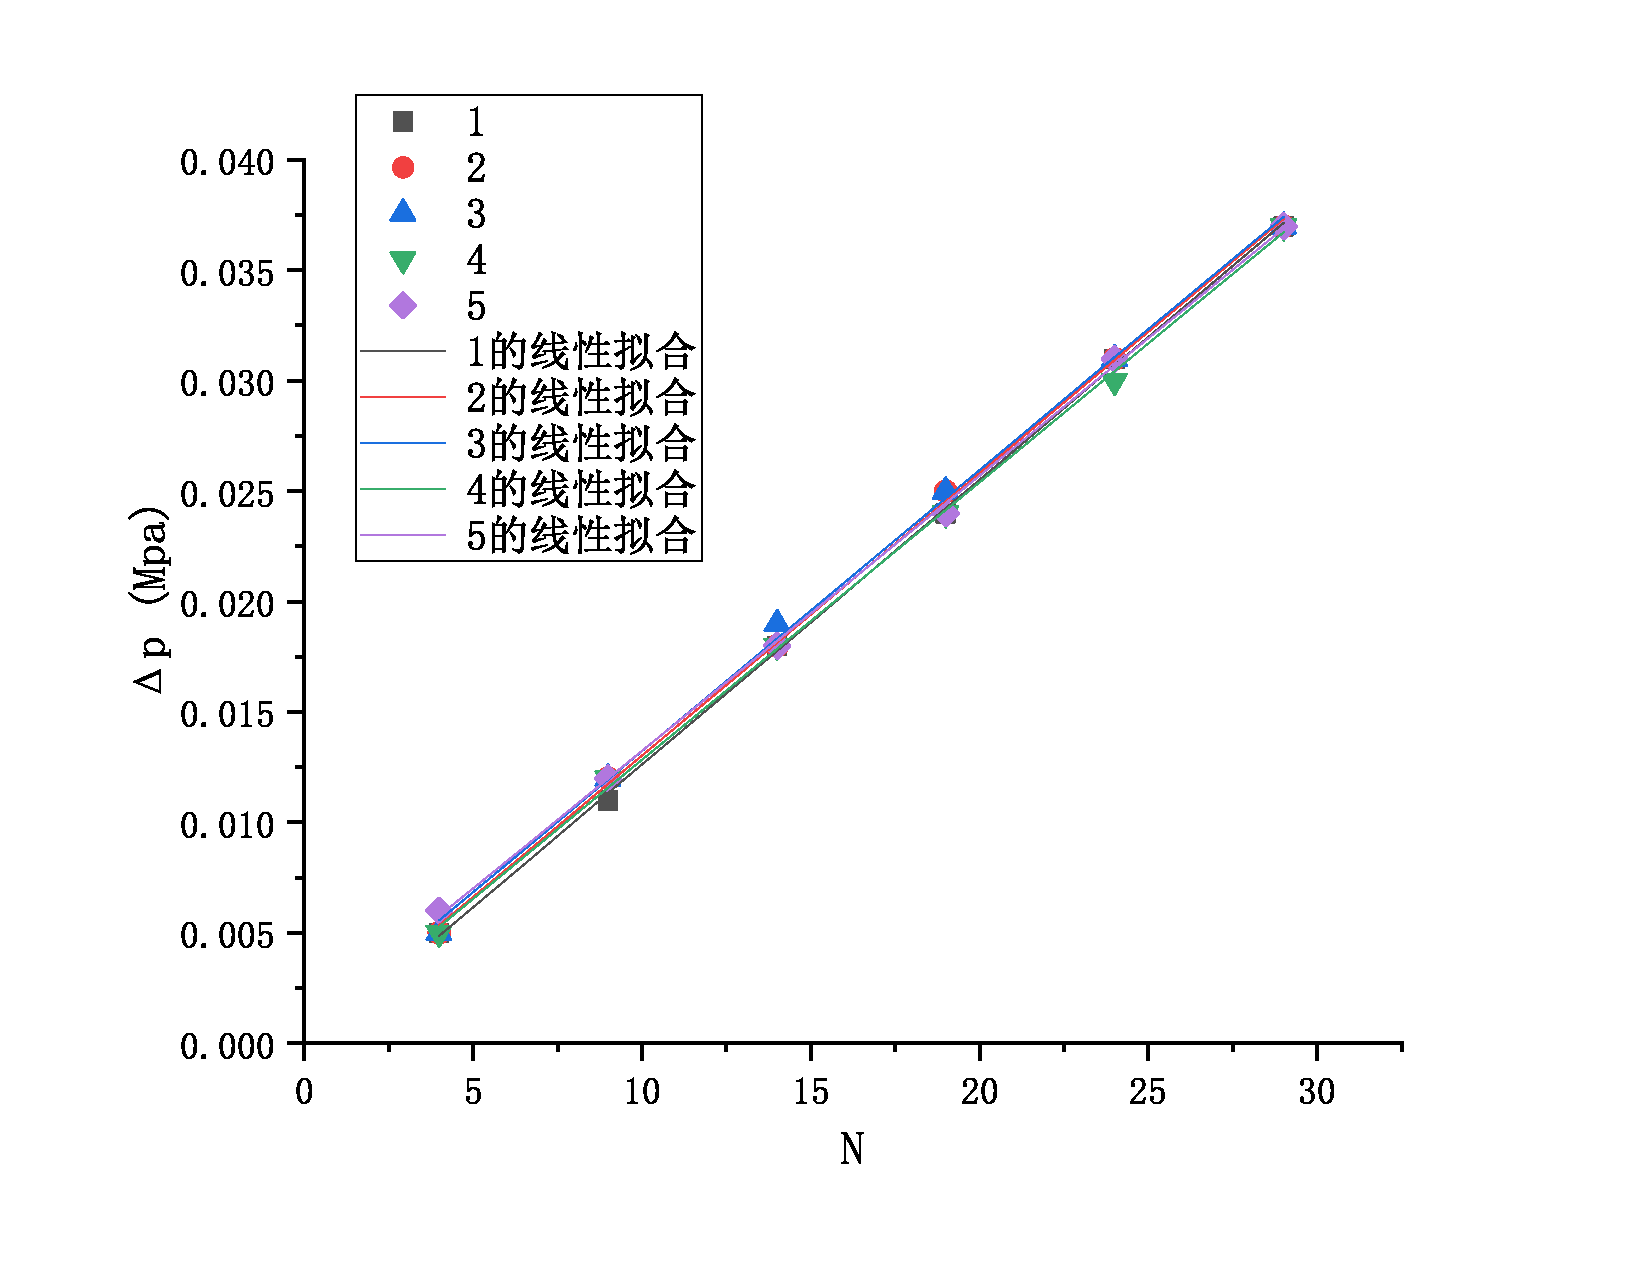
\includegraphics[width=.91\linewidth]{./figs/3.eps}
	\end{figure}
	利用表格数据计算得到:
	\[\frac{\Delta p}{N}=\left(0.00127\pm  1.798\times 10^{-5}\right) \operatorname{Mpa}\]
	代入公式(8)计算得到折射率:
	\begin{equation}
		n=1.000292
	\end{equation}
	与真值$1.000293$的绝对误差仅为$1\times10^{-6}$!,相对误差约为$1\times10^-4\%$!这已经是非常精确的测量结果。但是如果不使用这种数据拟合的实验处理方法,而是直接使用总的$\Delta N$除以总的$\Delta p$得到的折射率为$n=1.000289$,与真值之间的绝对误差为$4\times10^{-6}$,结果要稍微差一些。
	
	无论用哪种方法,得到的结果都相当精确,展现了迈克尔逊干涉仪虽诞生于19世纪,但在精密测量领域上仍有强大的实力。利用数据拟合处理实验数据,还能够使得测量值更加逼近真值。
	\subsection{夫琅禾费双缝干涉法}
	测量条纹改变10个后气压的改变,多次测量得到:
	\begin{table}[H]
		\centering
		\begin{tabular}{|c|c|c|c|c|}
			\hline
			$\Delta p(\operatorname{mmHg})$ & 172 & 172 & 171 & 174 \\ \hline
			& 170 & 172 & 172 &     \\ \hline
			$\overline{\Delta p}(\operatorname{mmHg})$&\multicolumn{4}{c|}{$171.9\pm1.2$} \\ \hline
		\end{tabular}
	\end{table}
	再利用公式(9)计算得到:
	\begin{equation}
		n=1.000281\pm0.000002
	\end{equation}
	不过上面的不确定度计算没有包含仪器自身的不确定度,仅仅只是非常简单的估计值。上面的测量平均值与真值之间的绝对为$1.2\times 10^{-5}$,相对误差为$0.0012\%$,要比前面迈克尔逊干涉仪得到的结果差不少。
	
	除了因为仪器本身结构导致机械误差要大一些,还有一点是因为在CCD显微仪上看到的条纹并不是太清晰,而且宽度较宽还并非规则的矩形,所以导致肉眼在测量时不是很容易判断条纹的移动。测量时使用的气压计为机械结构而不是电子传感器结构,而气压计的度数变化又较快,这又为准确读数带来了困难,所以最终误差较大。
	
	\section{结\quad 论}
	本次实验利用两种不同的干涉方法测定了空气的折射率,并且利用了数据拟合手段进一步减小了实验误差。最终使用迈克尔逊干涉仪得到的结果要比夫琅禾费双缝干涉法得到的结果好一个数量级。
	
	本次实验在数据处理上值得改进的一点是对不确定度的计算,因为仪器的不确定度没有给出,也不易估计,所以实验上仅仅只是给出了多次测量的统计标准差,并没有真正去计算结果的不确定度。另外,测量得到的结果都偏小,从公式(8)(9)来看只能是对气压的改变$\Delta p$的测量偏大,这需要通过改进气压的测量手段来减小这方面的误差\upcite{ref4},是力学测量上的问题。
	
	通过本次实验,重点是体会了为何迈克尔逊干涉仪在精密测量上有着如此强大的地位,并且通过思考,利用数据处理方法对实验最终精度给予了提升。气体折射率的测量是非常重要的,比如在真空计量上就有很大的应用\upcite{ref6}。
	
	\bibliographystyle{unsrt}

	\begin{thebibliography}{99}  
		\bibitem{ref1} 张萍,侯晨霞,宋金璠.综合设计性实验教学的研究与探讨一迈克尔逊干涉仪的拓展应用[J].实验技术与管理,2011 (8):157-159.
		\bibitem{ref2}李泽琴,宁长春,杨瑞等.认识和探测宇宙的基本方法介绍[J/OL].物理与工程:1-14[2023-12-30].
		\bibitem{ref3}杭乐斌,李雪梅.迈克尔逊干涉仪测量空气折射率实验中最佳间隔条纹数的探讨[J].大学物理实验.
		\bibitem{ref4}肖井华,红建强.干涉法测空气折射率的一点改进[J].大学物理,1993(04):32-48.
		\bibitem{ref5}[1]包力,毕胜楠.气体折射率测量方法的研究[J].吉林化工学院学报,2017,34(07):75-76+84.
		\bibitem{ref6}[1]许玉蓉,刘洋洋,王进等.基于气体折射率方法的真空计量[J].物理学报,2020,69(15):250-256.
	\end{thebibliography}
\end{multicols}

\end{document}
